% Options for packages loaded elsewhere
\PassOptionsToPackage{unicode}{hyperref}
\PassOptionsToPackage{hyphens}{url}
%
\documentclass[
]{article}
\usepackage{lmodern}
\usepackage{amssymb,amsmath}
\usepackage{ifxetex,ifluatex}
\ifnum 0\ifxetex 1\fi\ifluatex 1\fi=0 % if pdftex
  \usepackage[T1]{fontenc}
  \usepackage[utf8]{inputenc}
  \usepackage{textcomp} % provide euro and other symbols
\else % if luatex or xetex
  \usepackage{unicode-math}
  \defaultfontfeatures{Scale=MatchLowercase}
  \defaultfontfeatures[\rmfamily]{Ligatures=TeX,Scale=1}
\fi
% Use upquote if available, for straight quotes in verbatim environments
\IfFileExists{upquote.sty}{\usepackage{upquote}}{}
\IfFileExists{microtype.sty}{% use microtype if available
  \usepackage[]{microtype}
  \UseMicrotypeSet[protrusion]{basicmath} % disable protrusion for tt fonts
}{}
\makeatletter
\@ifundefined{KOMAClassName}{% if non-KOMA class
  \IfFileExists{parskip.sty}{%
    \usepackage{parskip}
  }{% else
    \setlength{\parindent}{0pt}
    \setlength{\parskip}{6pt plus 2pt minus 1pt}}
}{% if KOMA class
  \KOMAoptions{parskip=half}}
\makeatother
\usepackage{xcolor}
\IfFileExists{xurl.sty}{\usepackage{xurl}}{} % add URL line breaks if available
\IfFileExists{bookmark.sty}{\usepackage{bookmark}}{\usepackage{hyperref}}
\hypersetup{
  pdftitle={Manifestation of Spatial Inequality in Pune},
  hidelinks,
  pdfcreator={LaTeX via pandoc}}
\urlstyle{same} % disable monospaced font for URLs
\usepackage[margin=1in]{geometry}
\usepackage{graphicx,grffile}
\makeatletter
\def\maxwidth{\ifdim\Gin@nat@width>\linewidth\linewidth\else\Gin@nat@width\fi}
\def\maxheight{\ifdim\Gin@nat@height>\textheight\textheight\else\Gin@nat@height\fi}
\makeatother
% Scale images if necessary, so that they will not overflow the page
% margins by default, and it is still possible to overwrite the defaults
% using explicit options in \includegraphics[width, height, ...]{}
\setkeys{Gin}{width=\maxwidth,height=\maxheight,keepaspectratio}
% Set default figure placement to htbp
\makeatletter
\def\fps@figure{htbp}
\makeatother
\setlength{\emergencystretch}{3em} % prevent overfull lines
\providecommand{\tightlist}{%
  \setlength{\itemsep}{0pt}\setlength{\parskip}{0pt}}
\setcounter{secnumdepth}{-\maxdimen} % remove section numbering

\title{Manifestation of Spatial Inequality in Pune}
\author{}
\date{\vspace{-2.5em}2019-04-24T00:00:00Z}

\begin{document}
\maketitle

\hypertarget{introduction}{%
\subsection{Introduction}\label{introduction}}

According to the latest census data available globally, more than half
the world's population lives in urban areas. This, of course, is
influenced by how governments define `urban area' to be, as each nation
uses its own criteria of density, employment, land-use, etc. However,
one can agree that the proportion of dense, urban settlements is
increasing. (Satterthwaite 2002)

Cities are more than just a collection of people. They promote the
development of heterogeneity. Social interactions among dissimilar
groups break down traditionally rigid hierarchical boundaries such as
caste or race, and add a layer of complexity by introducing `class'.
This further complicates existing social stratification. (Wirth 1938)

Historically, spatial segregation in human settlements in India has been
along caste and religious lines. Caste also influences social and
material capital. Today with the introduction of `class', this spatial
segregation in metropolitan cities tends to manifest itself into `elite'
and `non-elite' areas. Using Mumbai as an example, Colaba is home to
some of India's wealthiest individuals, while Dharavi, less than 10
miles away is home to Asia's largest slum. (Sarpotdar 2017)

Caste-based discrimination has been outlawed since the adoption of the
current Constitution in 1950 and the Indian Penal Code. Despite
provisions for affirmative action, and social development programs aimed
at historically oppressed castes, they continue to face challenges in
accessing quality education, housing, health services, employment, and
public infrastructure. It should be noted, however, that regional
differences exist in the way each group is identified, and the intensity
with which discrimination occurs varies. (Zacharias and Vakulabharanam
2011) Dr.~B. R. Ambedkar, the principal author of the current
Constitution of India writes in his treatise `The Annihilation of Caste'
that caste is not only a division of labor but a division of laborers.
The relationship between caste and class in India is a close one, and
thus the two can seldom be considered two separate categories.

A large number of papers and research articles written on the state of
India's cities, the caste-system, social hierarchy, and economy exist.
These studies have historically been carried out on the back of smaller
sample-survey data both due to the lack of availability of higher
resolution data, and lack of computational capability. Thus, the dearth
in data has severely restricted the scope of researchers studying these
indicators at individual city and sub-city levels. Today with an
increase in the availability of digitized and tabulated high-resolution
data resources, quantitative research is becoming a possibility -- at
least in the largest metropolitan cities. (Zacharias and Vakulabharanam
2011) The 4 traditional metropolitan cities of Mumbai, Delhi, Chennai,
and Kolkata along with the three largest state capitals of Ahmedabad,
Hyderabad, and Bangalore tend to dominate any discussion of urban study.
However, with nearly five hundred cities in India with a population of
more than one hundred thousand we need to understand these cities'
individual patterns of growth, development, and networks. (Sarpotdar
2017)

\hypertarget{background-why-pune}{%
\subsection{Background: Why Pune?}\label{background-why-pune}}

Most large-scale urban level studies with a national or international
scope consider only the previously mentioned seven largest cities:
Mumbai, Delhi, Chennai, Kolkata, Hyderabad, Bangalore, and Ahmedabad.
Admittedly, these cities with a combined population of more than 80
million account for approximately twenty percent of the total urban
population of India. However, due to the vast size of India's
population, nearly 50 cities have a population larger than 1 million.
Pune is the 9th largest city by population, which according to the 2011
census stood at 3.12 million. (Census 2011)

Pune was one of the first cities in India studied from a lens of
segregation and social divisions (Mehta 1969). This and previous studies
by Gadgil in 1956 show that Pune is highly segregated, with clustering
based on caste and income. However, the city has undergone vast
transformations in the fifty-odd years since, with change accelerating
especially after the economic liberalization reforms of 1991, and as
such these studies are outdated and do not correspond to current ground
realities.

The history of settlement in Pune closely corresponds to that of many
other cities in India. Cities provided protection for their residents
during times of distress and political instability. Thus they attracted
upper-caste rural residents forming a very homogenous culture and
identity. Increasingly these cities required labor, thus contributing to
the migration of lower-caste groups to these cities. However, due to
spatial segregation, these migrants had to live in the city outskirts.
This pattern can be seen even today. Pune has grown in what can be
called concentric rings through the decades. Even today, the inner old
city core is dominated by upper-caste groups, surrounded by a diffused
ring, corresponding to the 20th-century expansion of upper-caste
residents with pockets of low-income lower-caste residents. (Mundhe and
Jaybhaye 2014)

Due to such similarities, Pune can serve as a `guinea-pig' of sorts to
understand spatial inequality in urban India, and how it's manifested
through transportation infrastructure, municipal investment, and
socio-economic factors such as employment, education, and health.

As such, we can examine these factors through the following broad
categories and methods of understanding:

\textbf{1. Socio-Economic Factors}

\begin{itemize}
\tightlist
\item
  Literacy, Fertility, employment, etc.
\end{itemize}

\textbf{2. Municipal Investment}

\begin{itemize}
\tightlist
\item
  Utilities, local roads \& streets, governmental services centers, etc.
\end{itemize}

\textbf{3. Transit Development \& Accessibility}

\begin{itemize}
\tightlist
\item
  Availability of transit options, usability \& functionality of transit
  options, etc.
\end{itemize}

We will elaborate on these factors in the following sections.

\hypertarget{datasets-we-are-using}{%
\subsection{Datasets we are Using:}\label{datasets-we-are-using}}

For the above-mentioned factors, we will be using these datasets:

\textbf{1. 2011 Primary Census Abstract for Pune City}

The decennial Indian census was first conducted in 1872, and regularly
since 1881. It collects data on various indicators on:

\begin{itemize}
\tightlist
\item
  Household Level: Housing quality \& material, number of rooms,
  ownership status
\item
  Individual Level: Age, gender, literacy, caste, economic activity,
  etc.
\end{itemize}

The census also provides separate data for Scheduled Castes (SC) and
Scheduled Tribes (ST).The Primary Census Abstract gives an overview of
some variables at the Ward level, which will be used in this research.

\textbf{2. Street Network Analysis Through OSMnx:}

OSMnx is a Python package used for downloading administrative boundaries
and street networks from the OpenStreetMap. It also allows one to
construct, project, visualize, and analyze complex street networks with
NetworkX.

We feed OSMnx with the shapefile of our census-wards for Pune and get
certain statistics for individual census-wards. These will be useful in
comparing street network patterns across neighborhoods with varying
socio-economic indicators. (Boeing 2017)

\textbf{3. PMPML Stops and Routes Dataset}

The Pune Mahanagar Parivahan Mahamandal Limited (PMPML) is the public
body entrusted with bus transit in the Pune and Pimpri-Chinchwad
Metropolitan Region. It was formed in 2003 after the two separate bodies
merged.

It maintains a fleet of 2045 buses servicing 2392 bus stops on 371
routes. The service suffers from mismanagement and an outdated and rigid
administrative structure. However, it is still used by 18.8\% of the
city's total road users and remains an important part of transportation
service.

This dataset contains information on stops, their location, and routes
servicing them, as well as whether they are part of the BRT (Bus Rapid
Transit) System or not.

\hypertarget{socio-economic-factors}{%
\subsection{Socio-Economic Factors}\label{socio-economic-factors}}

A large part of the character of a citizenry can be understood by
looking at socio-economic and health indices. These make us privy to
quality of life indicators such as education levels, fertility rates,
household sizes, sex ratio, and employment types.

Scheduled Castes and Scheduled Tribes are classifications made for
administrative purposes, they group underprivileged communities for a
wide variety of affirmative action programs and HDI improvement schemes.
These groups are generally considered minorities and are such in Pune.
It would be interesting to see how their proportions are manifested by
census-wards in Pune.

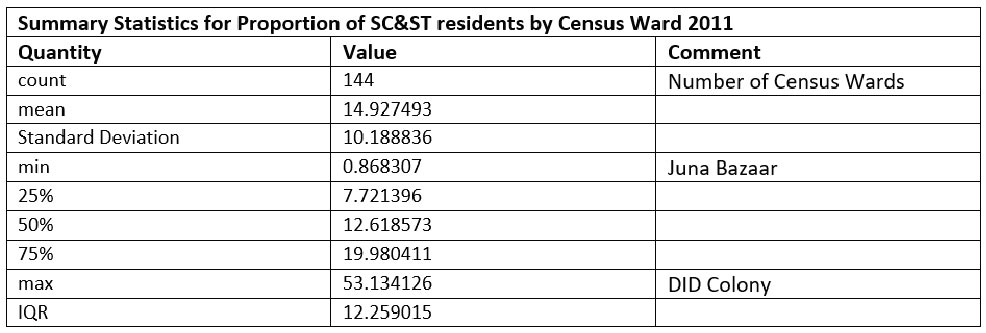
\includegraphics{/img/project/asa/sumstats_tbl_scst_prop.jpg}

We proceed to classify a ward as either majority dominant, or minority
dominant. Here, we see that the median value of SC\&ST proportion in a
census-ward is 12.618\%, and the Interquartile range is 12.259\%. We
take their total (24.877\%) as a dividing line between majority dominant
wards, (SC\&ST proportion less than 24.877\%) or minority dominant wards
(SC\&ST proportion more than 24.877\%).

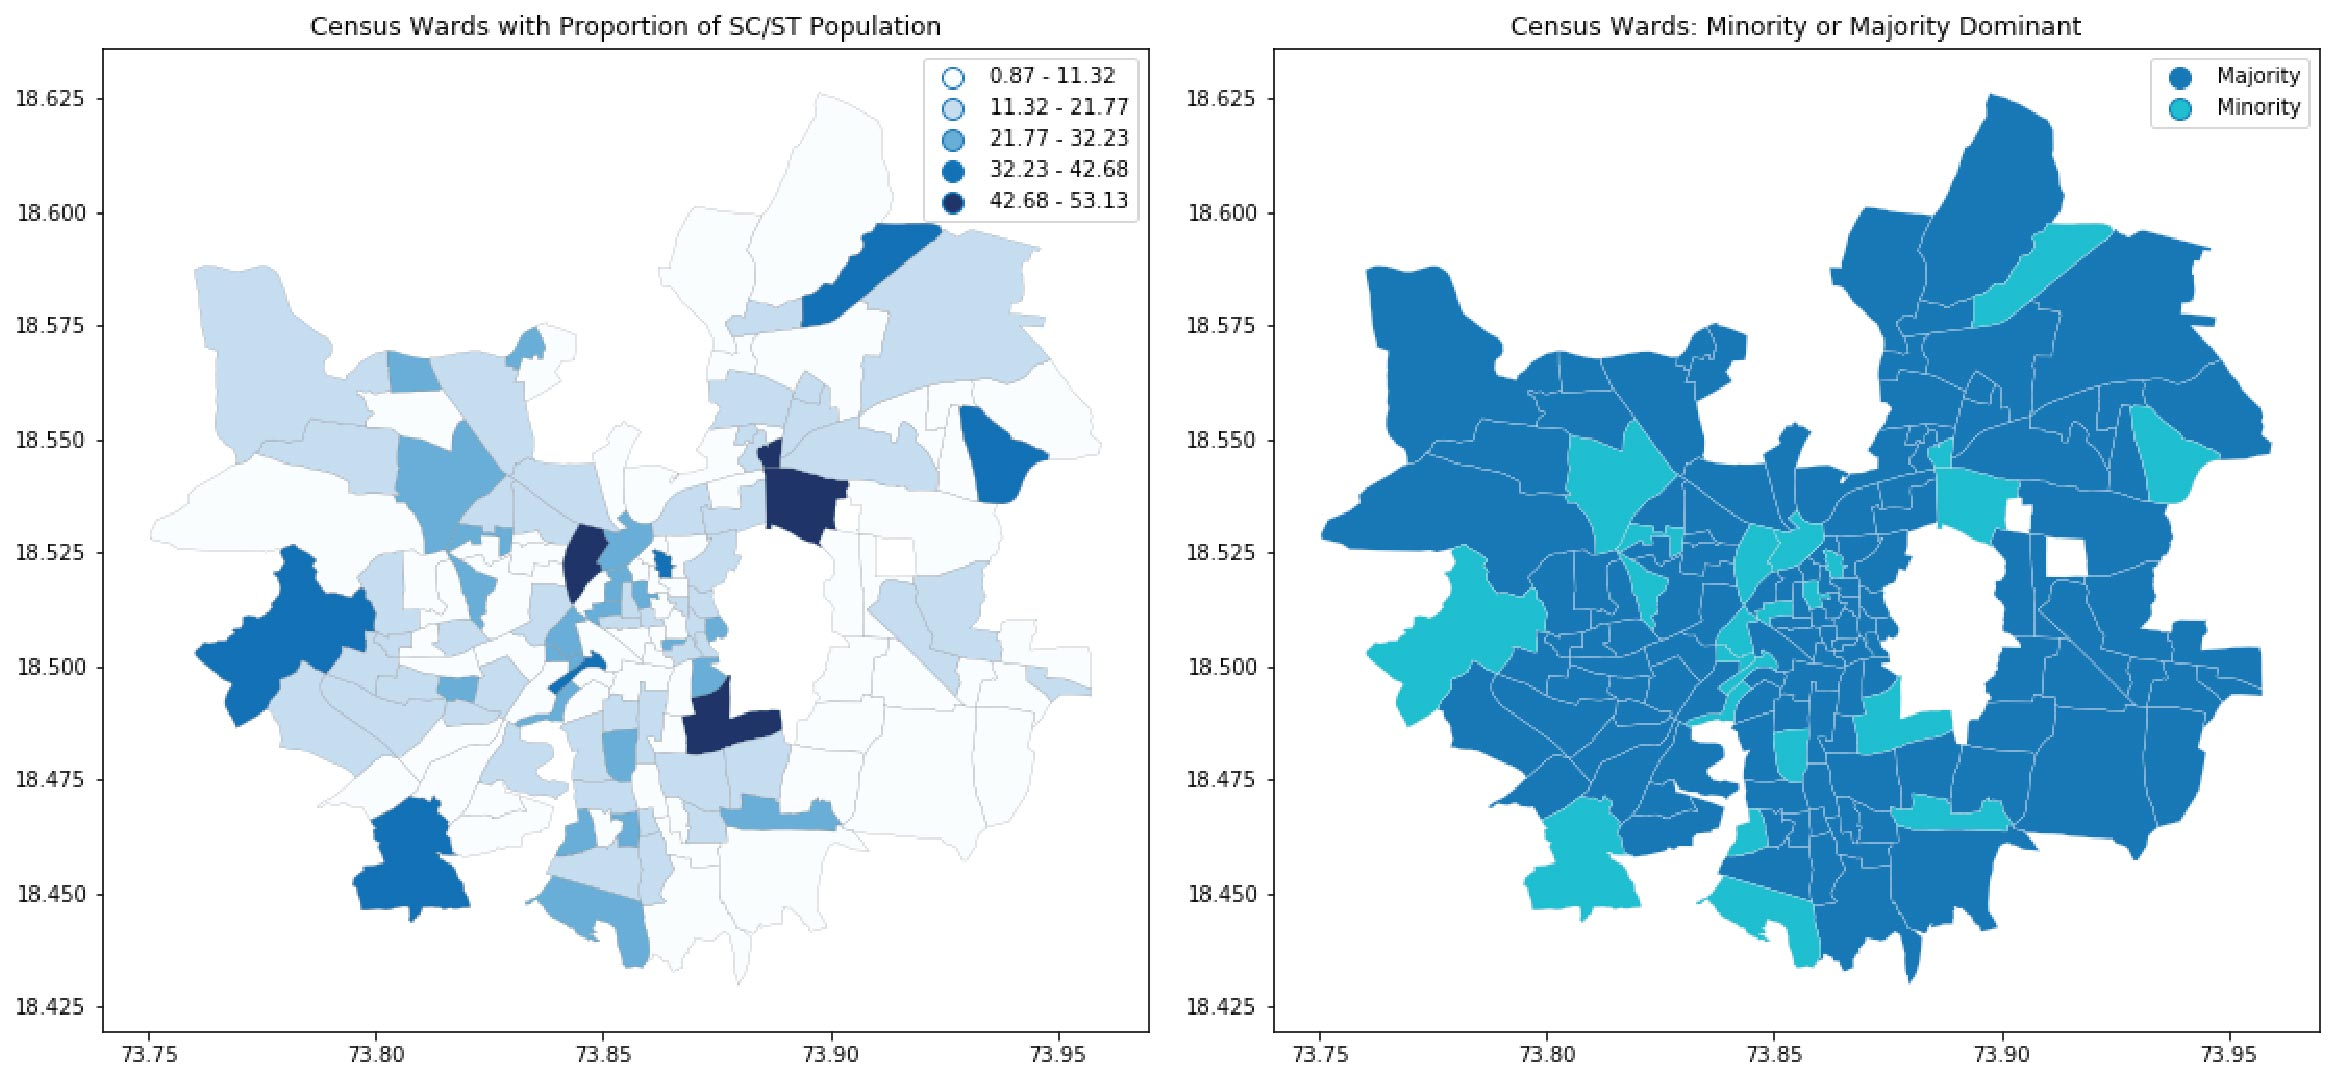
\includegraphics{/img/project/asa/scst_prop.jpg}

\hypertarget{literacy-rate}{%
\subsubsection{Literacy Rate:}\label{literacy-rate}}

Although universal access to education is guaranteed in the Indian
Constitution, it is not always the case. As might be obvious, SC\&STs
have been historically denied access to education, and even today, their
literacy rates remain well below that of dominant and privileged groups.
We can view this to be evident from a scatterplot, by comparing a ward's
literacy rate with its proportion of minority population.

Here, we see a visible correlation between literacy rate and the
proportion of SC\&ST residents of a ward. The literacy rate also affects
what kind of employment a person can get in their life, thus compounding
problems related to employability, and skill development. The Primary
Census Abstract also provides information on whether a person is
employed full-time, or is marginally employed.

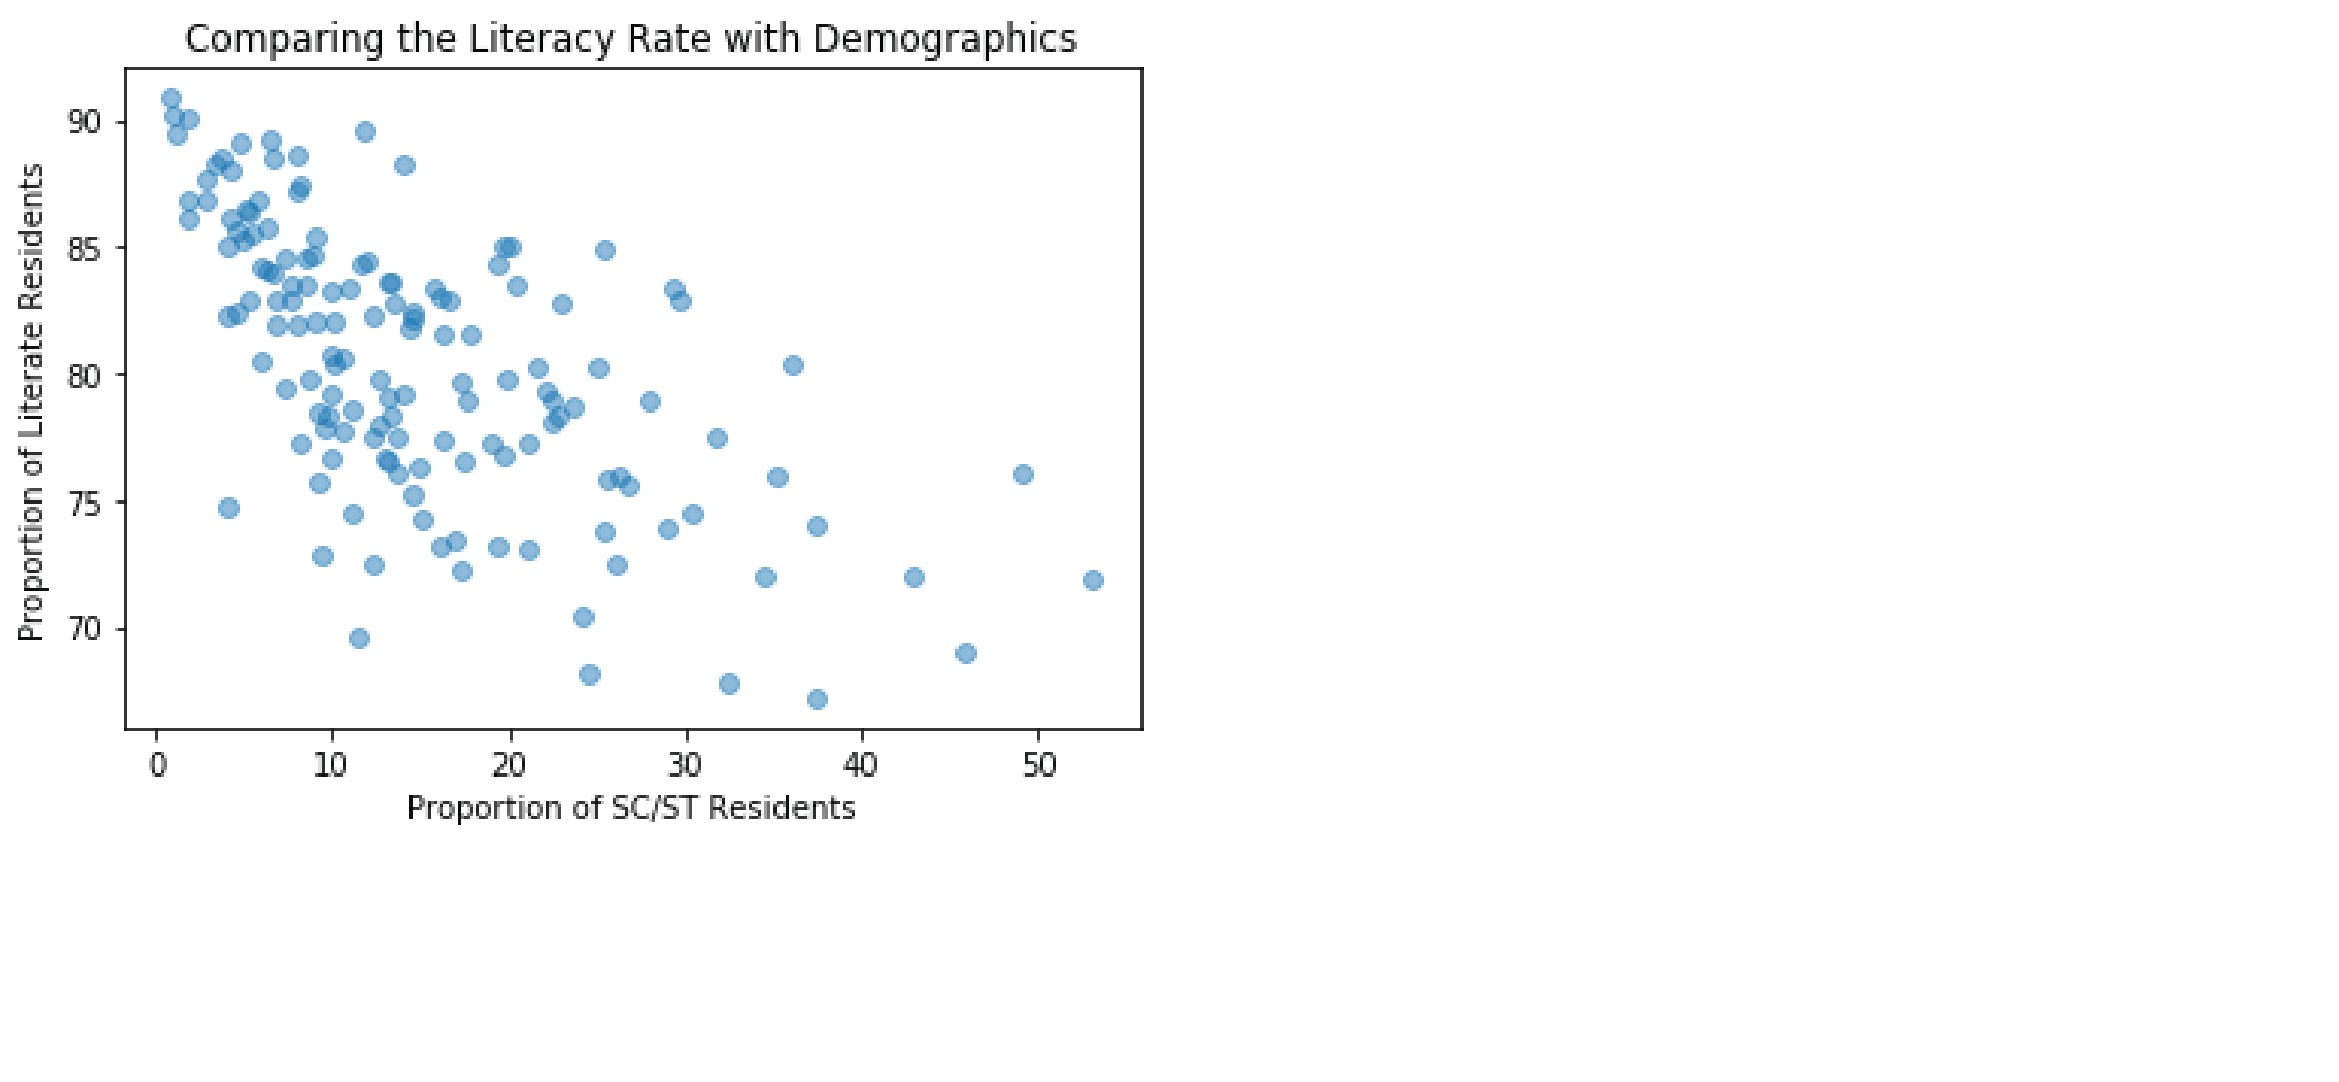
\includegraphics{/img/project/asa/literacy.jpg}

\hypertarget{marginal-employment}{%
\subsubsection{Marginal Employment:}\label{marginal-employment}}

A person with marginal employment has fewer chances of economic
security, and social stability. Marginal workers are those employed for
less than 6 months of the year. This results in a lower and less regular
source of income. This could be `part-time work', contractual daily-wage
or intermittent manual labor. According to data from 2009, 87.8\% of the
SC\&ST marginal worker population nationwide falls in the `Poor \&
Vulnerable' category, whereas this count is only 54\% for non-SC\&ST.
(Harriss-White and Prakash 2010) This shows that marginal work has a
caste factor. We can also see how this correlates with the literacy rate
in the above graph.

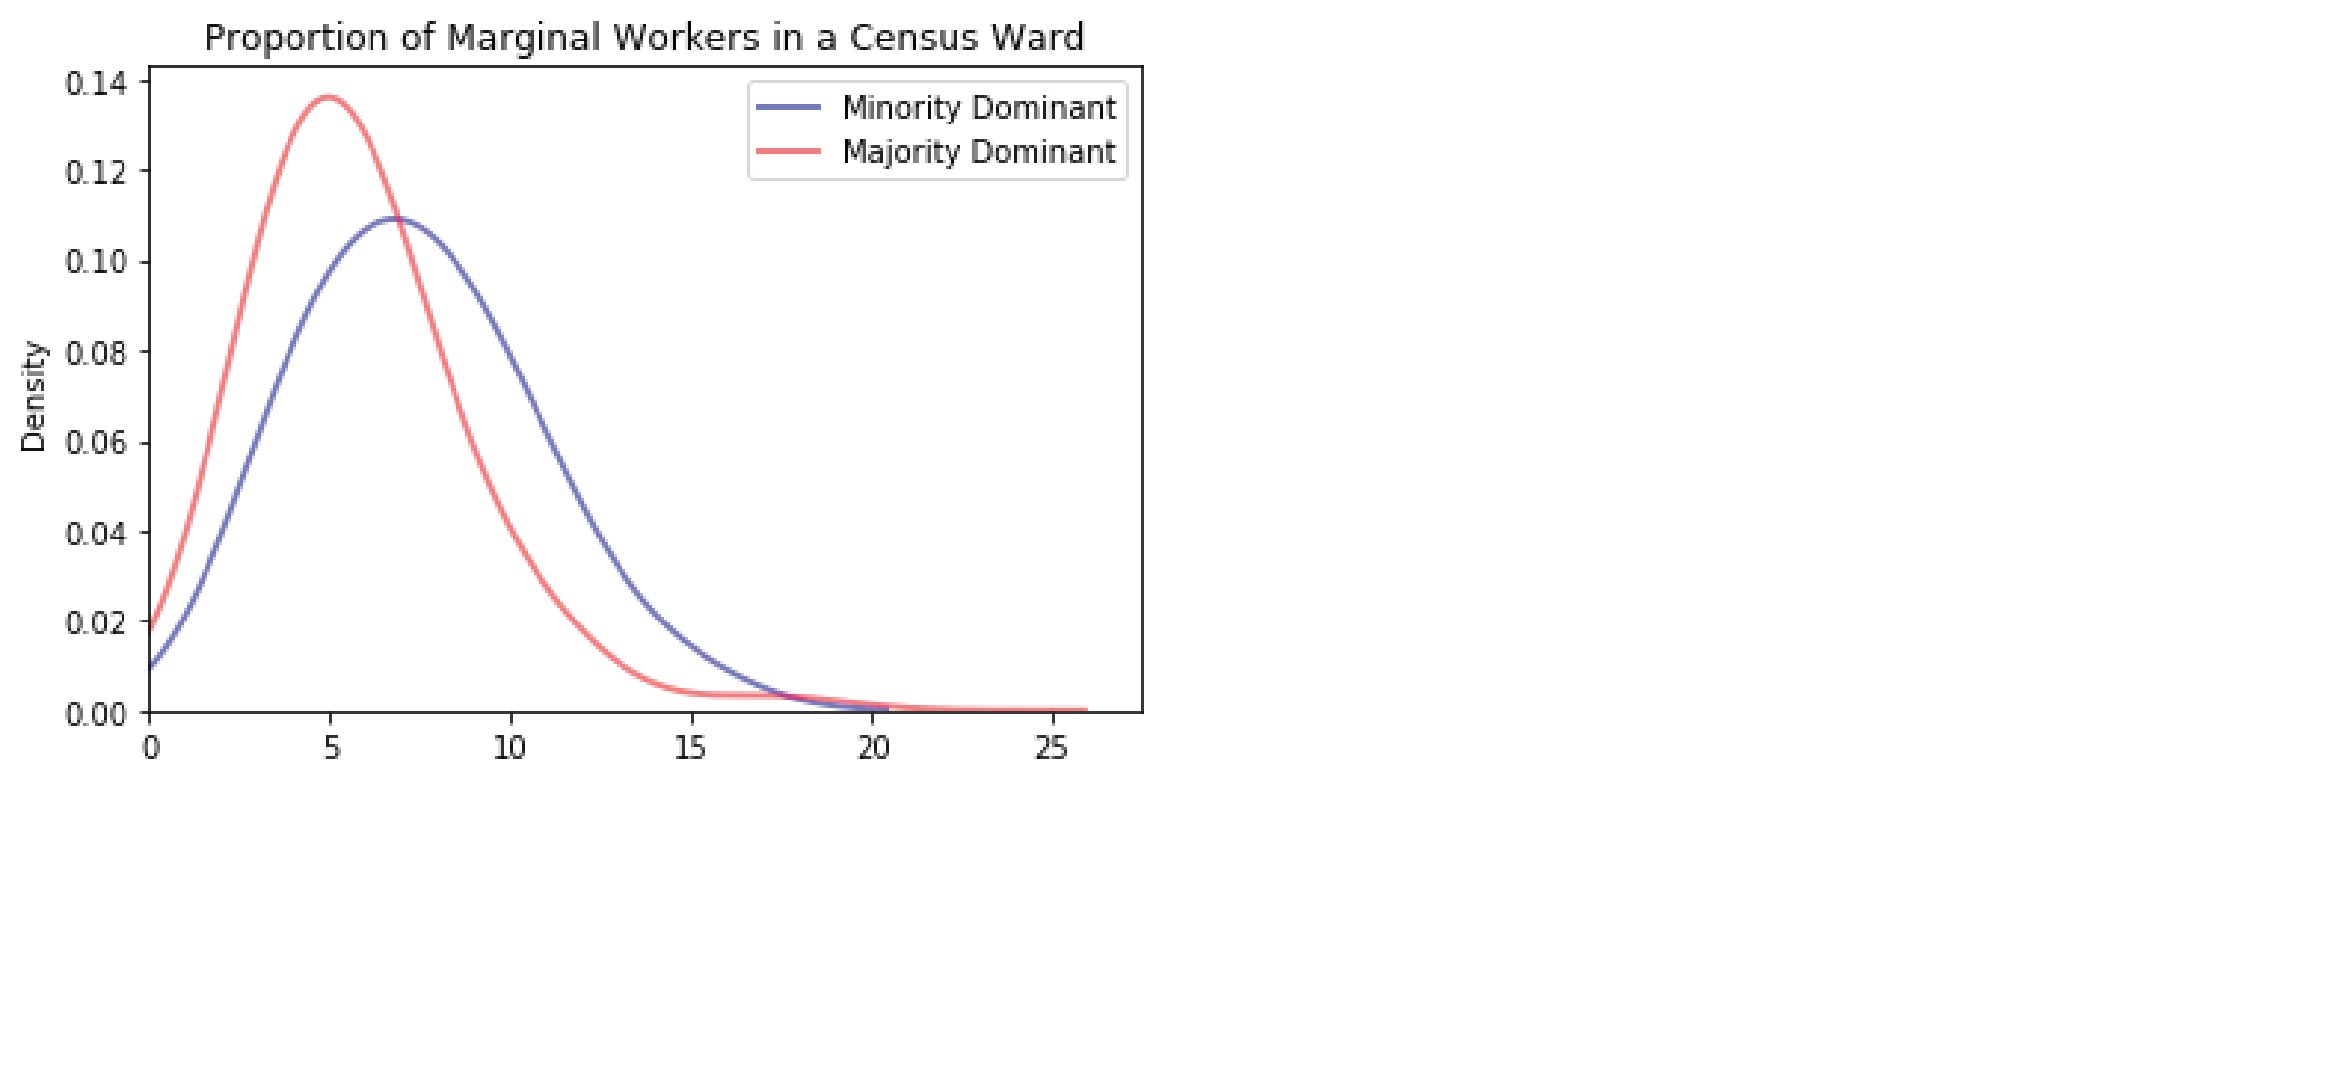
\includegraphics{/img/project/asa/marg_work.jpg}

With a difference in means t-test, we see that minority-dominant
census-wards tend to have a larger proportion of workers employed in
marginal work as compared to majority-dominant wards. With a p-value of
0.024, we see that the difference in means is statistically significant.

7 = minority dominant

5 = majority dominant

\hypertarget{municipal-investment}{%
\subsection{Municipal Investment}\label{municipal-investment}}

Funding for municipal investment in public infrastructure comes from
municipal wards through municipal level taxes, property taxes, and other
cesses aimed at infrastructural development and maintenance. An
interesting way to examine municipal investment is through road density.
Disadvantaged areas in Pune tend to be informally settled with fewer
municipal services. How road networks compare across various
neighborhoods may throw light on whether this holds true or not.

We used the OSMnx package in Python to get details of the street network
in each census-ward. The pattern of development closely follows the
general population density. When we compare by the proportion of SC\&ST
residents, we do not see any visible correlation.

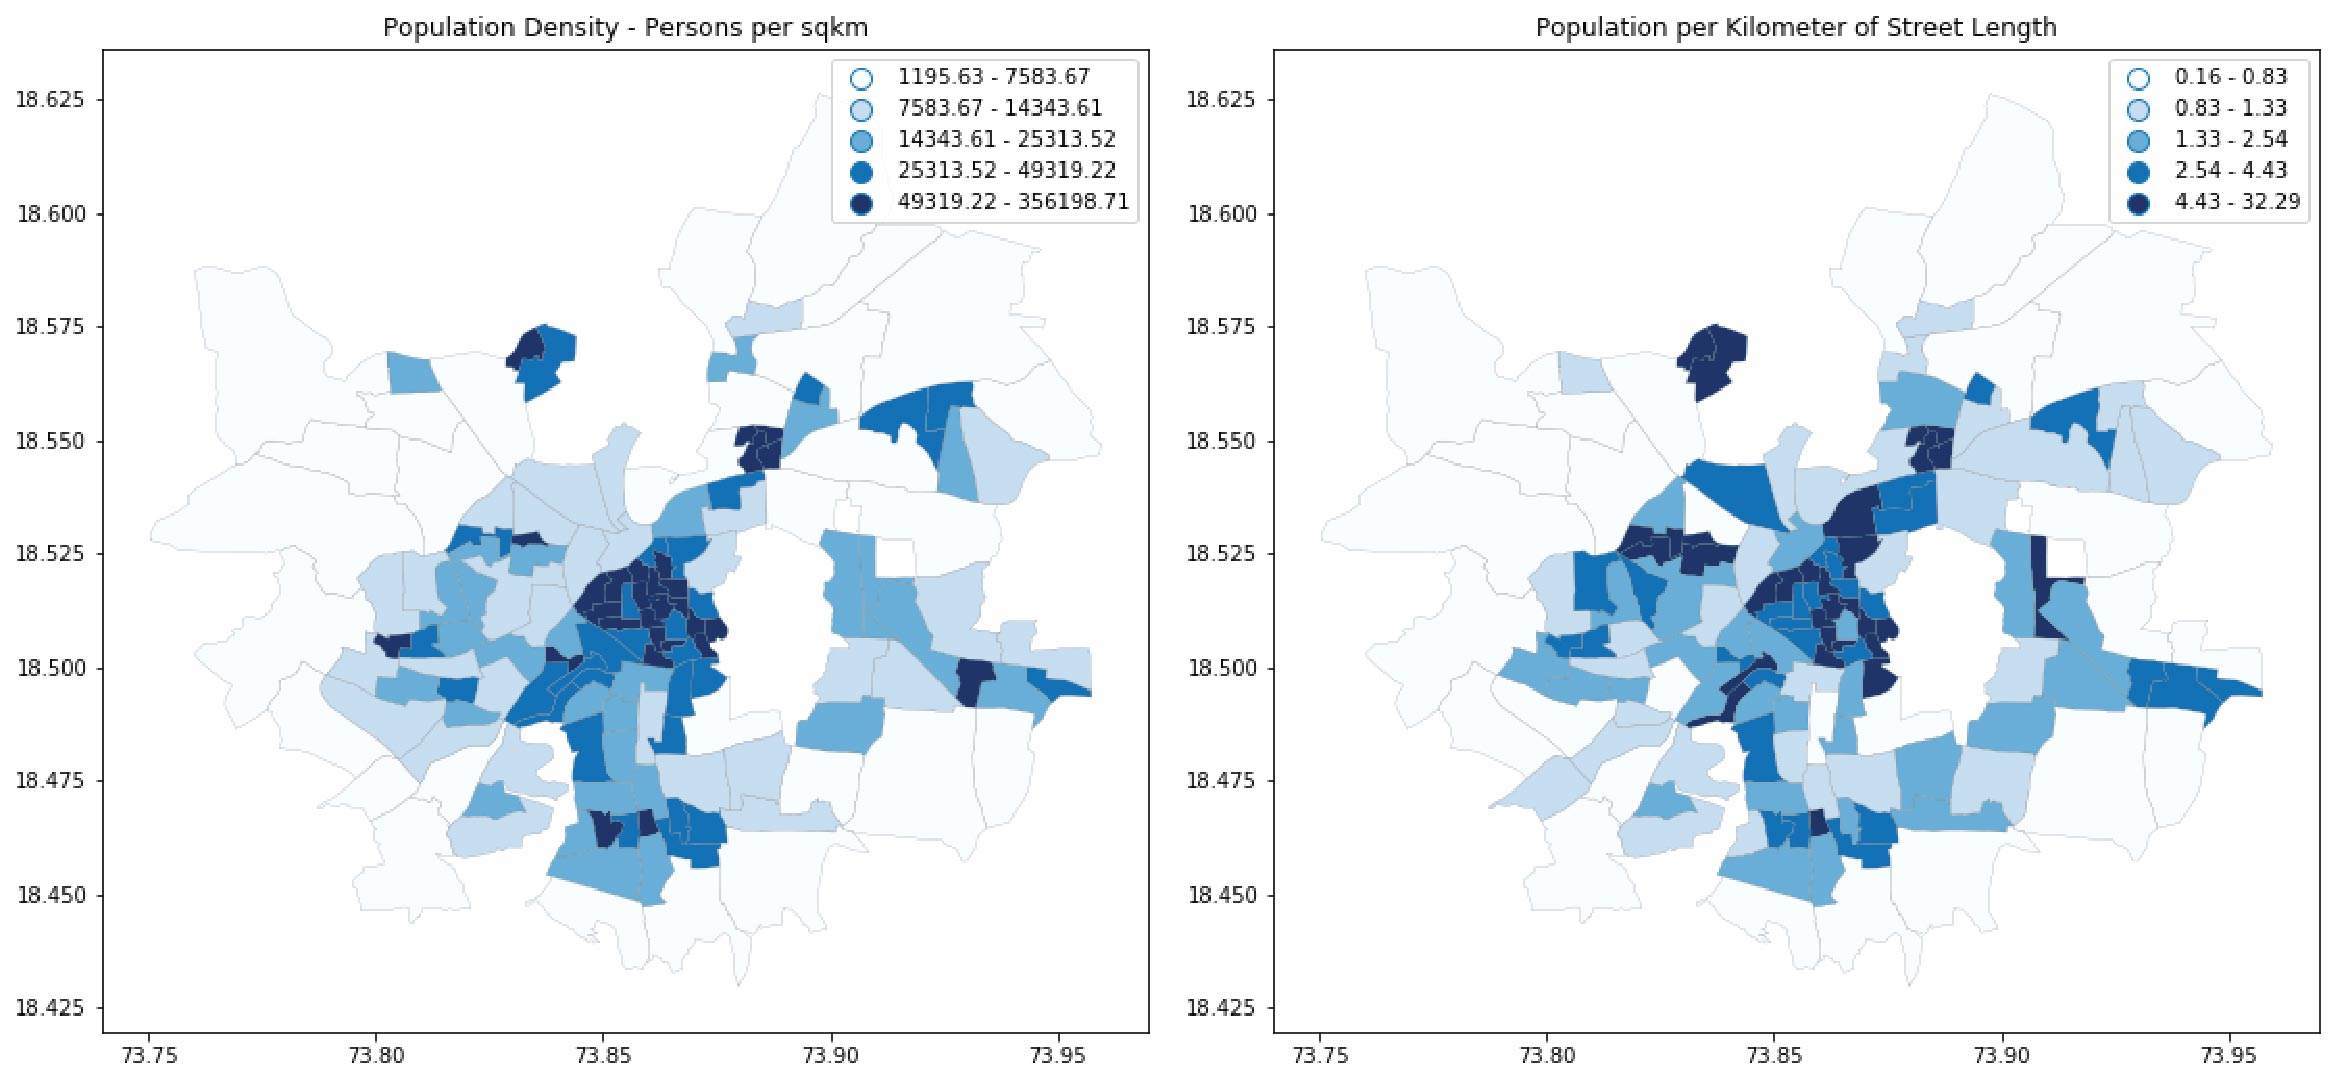
\includegraphics{/img/project/asa/pop_dens.jpg}

Data in the above maps are classified by 5 quantiles. We see that the
street length density and population density is comparable, with a few
differences. Thus, we can say that three kinds of instances occur when
comparing these two maps:

\textbf{1. Equally Comparable:}

The Difference in ratios equal to 0

\textbf{2. Population Density higher than Street Length Density}

The Difference in ratios more than 0

\textbf{3. Population Density lower than Street Length Density}

The Difference in ratios less than 0

When we visualize this by comparing the normalized ratios of the two
values, we get the following:

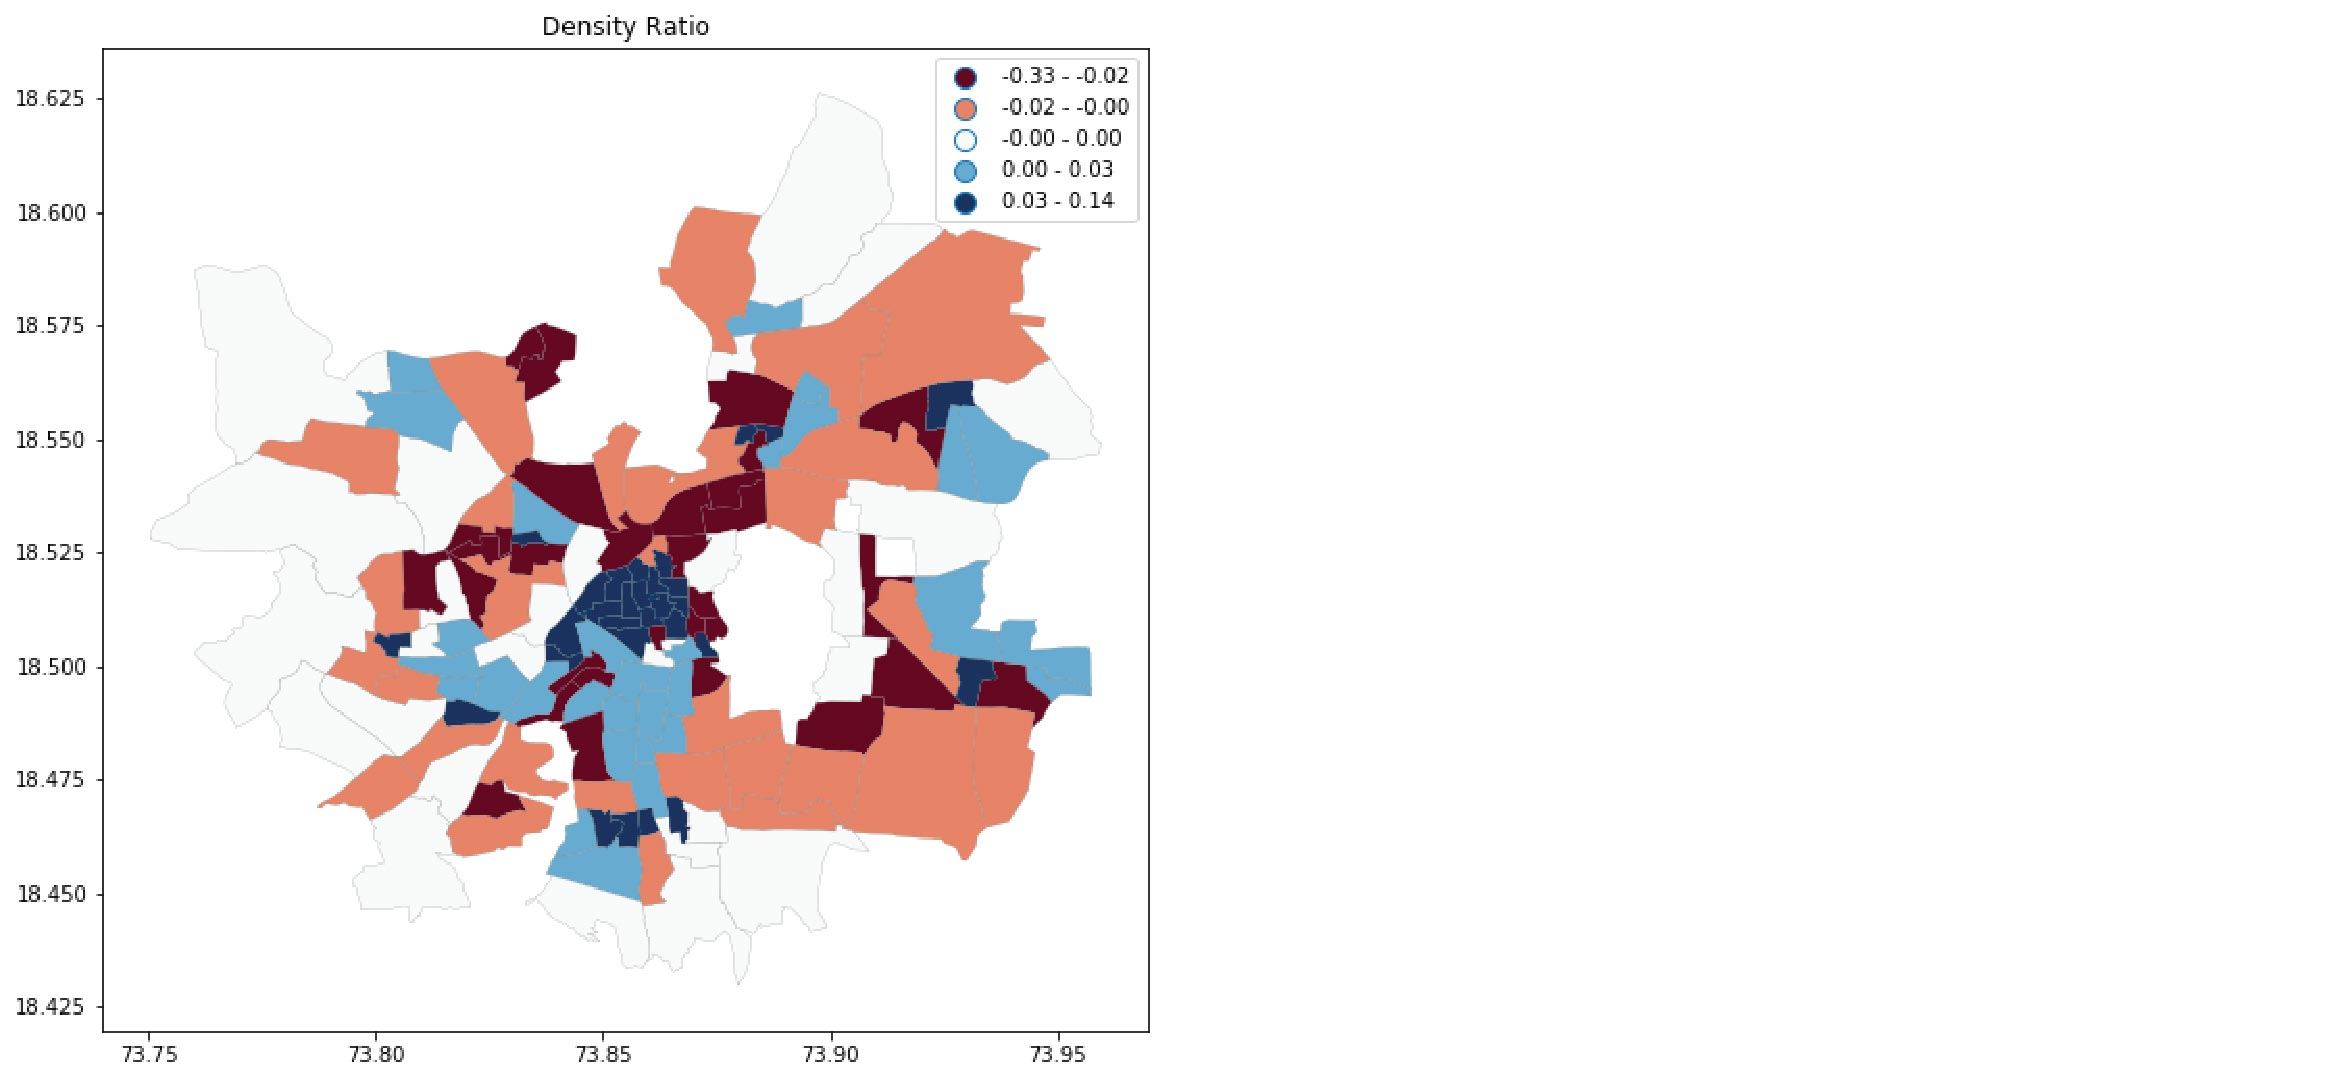
\includegraphics{/img/project/asa/dens_rat.jpg}

\textbf{1. Equally Comparable: (ratio = 0, grey)}

We can understand the ratio between population density and road density
is equal, i.e.~as one would expect it to be for a given ward in Pune of
any density. Much of the western areas of the outer periphery is in this
category, as areas just abutting the inner core.

\textbf{2. Population Density higher than Street Length Density (ratio
\textgreater{} 0, blues)}

We can understand this to mean that the ratio is imbalanced towards
having more people than one would expect to be for a given ward in Pune
of any density. This is most evident in the historic inner core, as well
as certain pockets in the central peripheral areas.

\textbf{3. Population Density lower than Street Length Density (ratio
\textless{} 0, reds)}

We can understand this to mean that the ratio is imbalanced towards
having fewer people than one would expect for a given ward in Pune of
any density. This can be observed largely in the eastern half of the
city, as well as areas just to the north. This area houses the
Agricultural College, as well as Koregaon Park -- a low-density wealthy
neighborhood with large single-family lots.

\hypertarget{transit-development-accessibility}{%
\subsection{Transit Development \&
Accessibility}\label{transit-development-accessibility}}

Accessibility to transportation has long been considered to have an
effect on quality of life indicators such as health, education, and
income. (Syed, Gerber and Sharp 2014) Communities with limited access to
roads and transportation options have limited ability to integrate with
the outside world. (Kumar and Karvajal 2017) In urban areas, this often
translates into residents of neighborhoods with underrepresented
populations not having equitable access to the city's transit system,
thus making it difficult for them to access employment, schooling, and
healthcare.

In dense transit-rich areas with a higher rate of transit dependence,
commute is an important indicator of quality of life. Pune, however, has
a low transit dependence at 18.8\%, and private vehicle users (2 and 4
wheeled vehicles) account for 46.9\% of road users.

Vehicle ownership is expensive in not only buying the vehicle but also
maintaining it. The modal share of pedestrians can explain this:
pedestrians account for 33.2\% of all trips. (Parisar 2012-13) With a
goal of increasing non-personal modes of transport to a combined total
of 90\% by 2040, we can assume that the Pune Mahanagar Parivahan
Mahamandal Limited (PMPML) which looks after transit in the Greater Pune
Area is looking to invest in transit.

The PMPML data includes information on the following key points:

\textbf{1. Route ID --} the unique identifying number for a given route

\textbf{2. Stop ID --} the unique identifying number for a particular
stop on a particular route. A particular stop name may feature multiple
times in the dataset and will be associated with multiple stop IDs
depending on how many routes it is covered in.

\textbf{3. Stop Name --} Unique name for each stop. Is repeated as many
times it is associated with a route.

*4. Latitude and Longitude --** Geographic coordinate points pair.

\textbf{Interesting values we can derive from this could be:}

\textbf{1. Stop Density:} How many stops per ward, or population per
stop for a given ward

\textbf{2. Stop Usability:} How many lines pass through a particular
stop?

To understand these two values, we considered joining the PMPML dataset
with the Census-Ward dataset. As such, we got two interesting values --
Stops count per ward and the median count of bus lines passing through a
bus stop in a given ward.

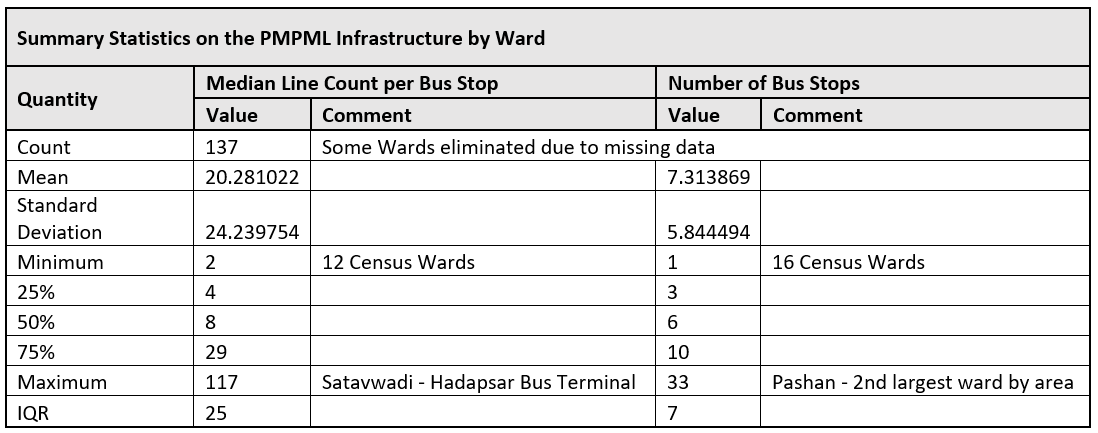
\includegraphics{/img/project/asa/pmpml_summstats.png}

When we compared the density of a census-ward with the median number of
bus lines passing through its bus stands, we get the following result:

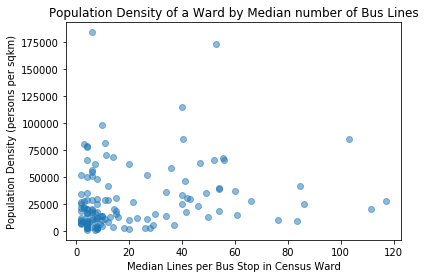
\includegraphics{/img/project/asa/transit_x_density.png}

We see that most census-wards have a population density of fewer than
25,000 residents per square kilometer. They also seem to have less than
10 lines per stop. The census-ward with the highest density recorded
also seems to have a lower median line count per stop at around 10. The
ward with the highest median line count per stop seems to have a low to
moderate density. This may be due to the reason that the ward
(Satavwadi) is the location of Hadapsar Gadital -- a bus terminal and
depot. As such, it is not deviating from what one would expect.

One should note, that the absurdly high levels density values seen here
are a distortion because of the small areas of the wards, as such, they
may not `feel' as dense as the numbers may seem to indicate.   We map
our two datasets: the PMPML points data, and the Census Polygon data,
with the following variables:

\textbf{1. From PMPML: Lines through a Stop}

This will give us an idea of how `useful' a particular stop is, how many
lines can one take from that stop. This is a good indicator of how far
one can go without needing to change to another line or vehicle.

\textbf{2. From the Census data: Proportion of SC\&ST residents}

As discussed, we would like to see how bus stops are placed with regard
to an area's proportion of minority residents.

Even though the PMPML's service area goes beyond the Pune Municipal
Corporation (PMC) area limits, we are showing only the area under the
PMC as this is the scope of our study.

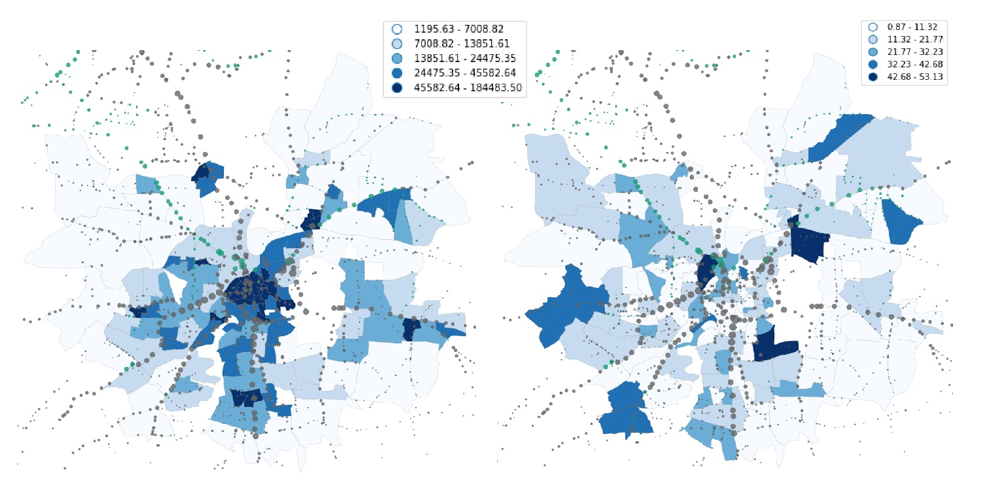
\includegraphics{/img/project/asa/busnetwork_bylanddensity.png}

Stops in the central parts tend to have the most lines served. We also
see key routes heavily serviced, with `frayed' ends marked with smaller
circles. This is indicative that many lines are similar for most of the
journey, and only the last and first few stops are different. This is a
very common and predictable pattern for a radial city.

We also see in the map on the right, the most heavily SC\&ST
proportioned wards do not have many well-serviced bus stops. The major
corridor lines have a very low proportion of SC\&ST residents.   \#\#
Cross-comparing our data:

We have looked at each dataset individually, and compared each one to
the other in some way to gain an understanding of how Pune works in the
three ways we aimed to examine it:

\textbf{1. Socio-Economic Factors:}

We understand the social layout of Pune and understood where there is a
dominant population of majorities and minorities in the city. We also
saw how economic activity is spread across the two social groups by
comparing marginal low-output activities.

\textbf{2. Municipal Investment:}

We understood how the street network changes and is laid out in each
census-ward. We also checked how the density of population and streets
compares against each other. What areas have the expected density, and
which do not (higher or lower).

\textbf{3. Transit Infrastructure:}

We see how the PMPML is spread across the city, and how areas are
served, depending on the population, and density.

After seeing all these insights, we further check for observable
correlations across these three datasets. As explained in the
introduction, the groups classified as SC (Scheduled Caste) and ST
(Scheduled Tribes) are among the most socially and economically
disadvantaged in India. After looking through the data, and the study we
conducted, the following indicators felt interesting to examine as
predictors of a ward's SC and ST proportion:

\textbf{1. The Proportion of Literate Residents:}

This is an important factor to consider. An illiterate person has fewer
economic opportunities, and consequently lower spending power. In Pune,
where only 18.8\% of the population uses public transport, bus nearly
33\% walk, we can guess that the cost of a bus ticket or pass may be
prohibitively expensive for at least some of those who are exclusively
pedestrian.

\textbf{2. Street Density:}

Informal settlements, also called slums, tend to have fewer `legitimate'
roads, leading to poor quality access paths with insufficient
asphalting, footpaths, or other street infrastructure. A
disproportionate number of SC\&ST citizens form the poorest sections of
society and have a higher likelihood of residing in these settlements.
As a result, this would be an interesting variable to consider.

\textbf{3. Population Density:}

Ideally, a denser area of the city would see a larger concentration of
services as well. How this compares to other factors will be interesting
to see.

\textbf{4. Number of Bus-stops:}

A larger number of bus stops in an area gives a larger spread of areas a
user/commuter can travel without needing to change lines/vehicles. This
gives better access to larger parts of the city.

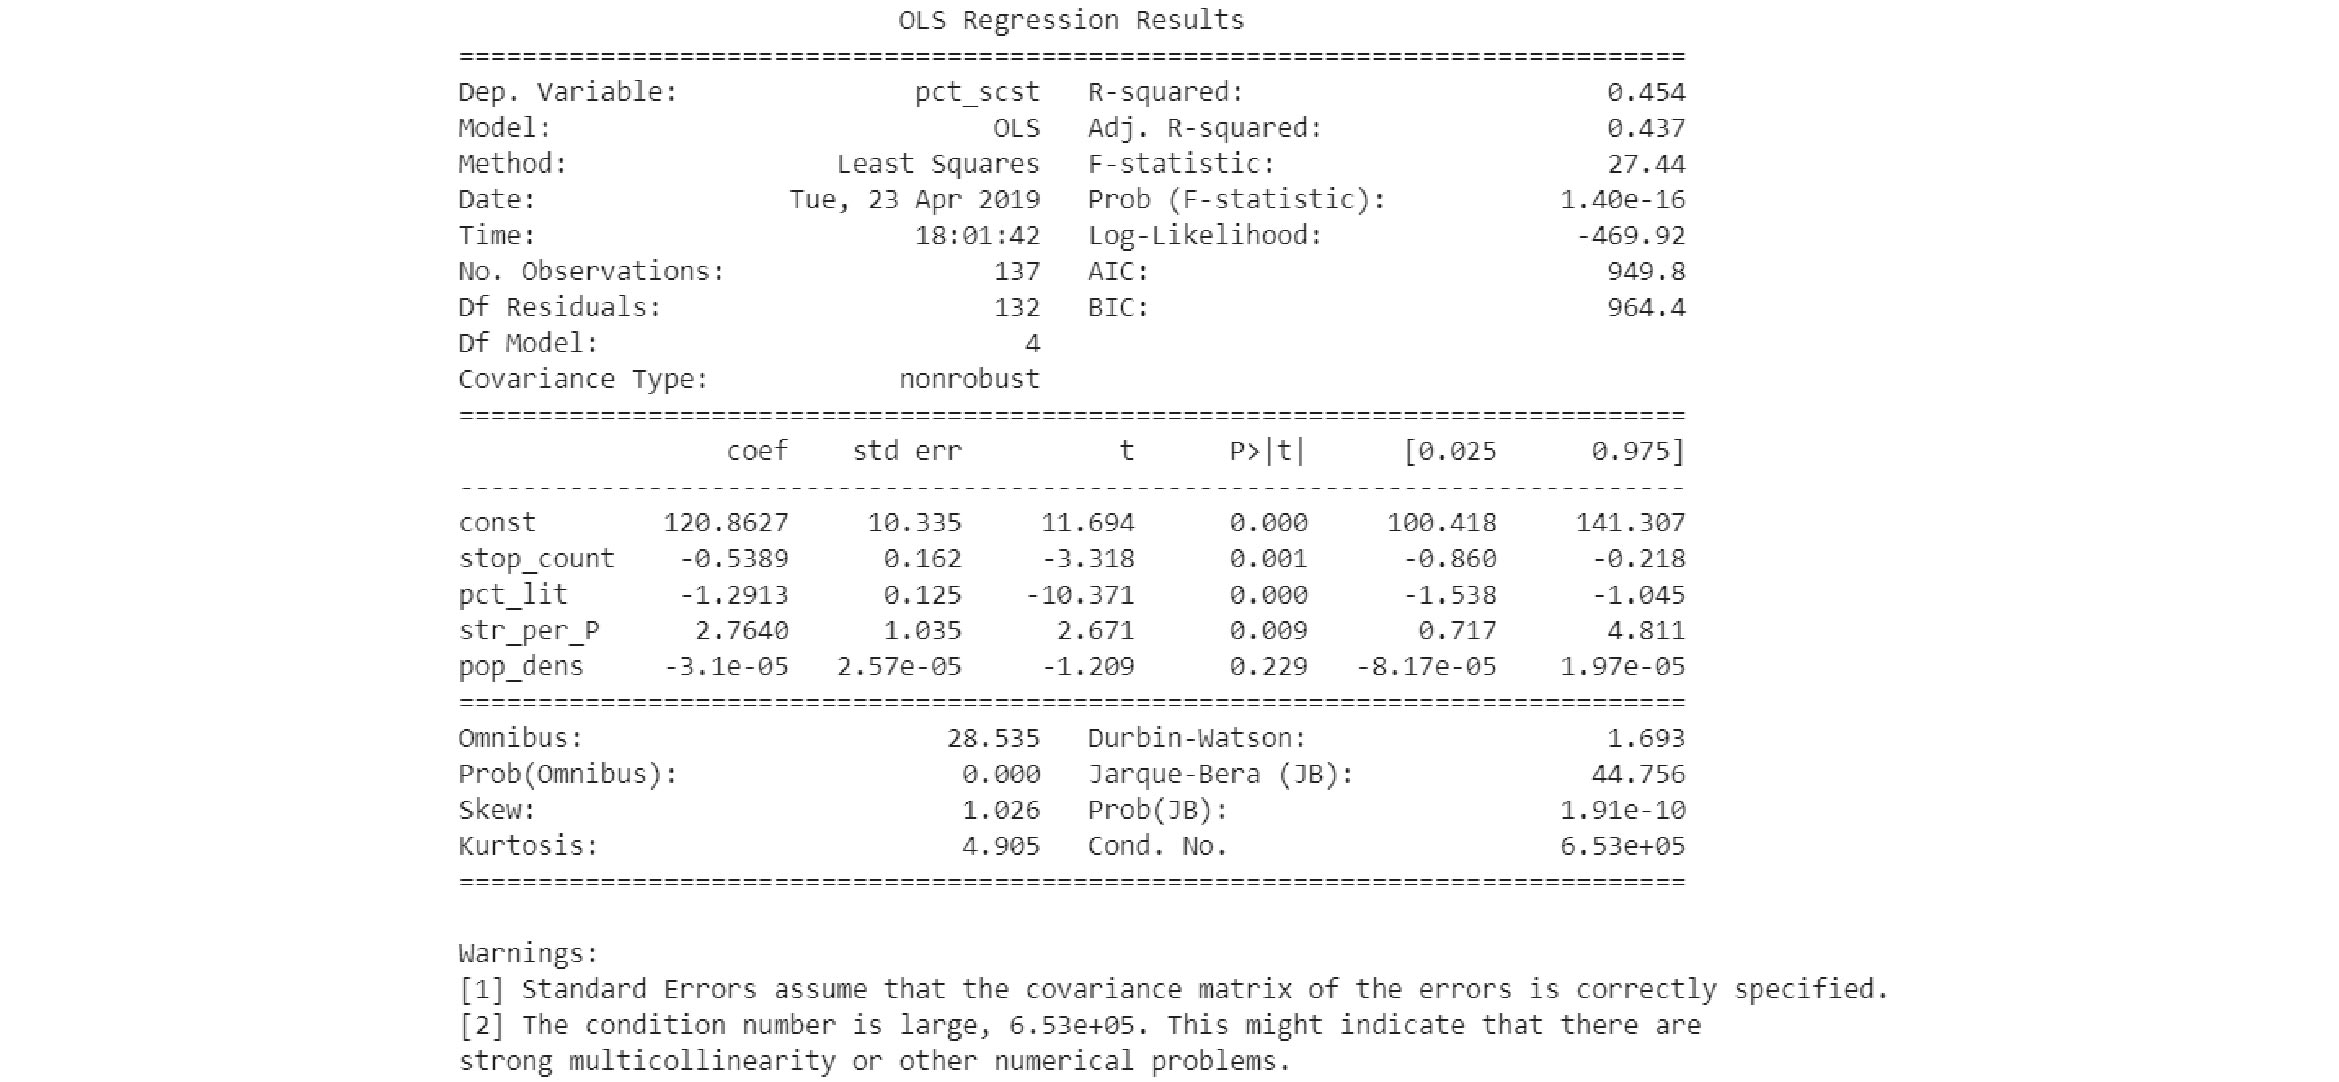
\includegraphics{/img/project/asa/ols_reg.jpg}

The p-value for stop count, street length per person, and proportion of
literate persons is very low. This indicates that they are influential
variables in determining a census-ward's proportion of SC\&ST residents.
Initially, it may be surprising that population density is not an
influential variable. One must remember that the core dense areas of the
city have a significantly low proportion of SC\&ST residents. As this
regression is based only on data from Pune, we cannot with conviction
apply it to other cities with a different socio-spatial structure.

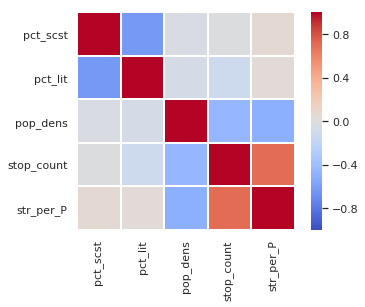
\includegraphics{/img/project/asa/correlation.png}

The R-squared value of 0.454 is indicative that these factors explain
45.5\% of the variance seen in the proportion of SC\&ST residents in
Pune.

When we do a correlation, we see a large negative correlation between
proportion SC\&ST and literacy rate.

Another interesting correlation is between street length per resident
and the bus stop count per ward, in that they are positively correlated.

We also see that a higher stop-count is correlated with a lower
population density. This seems counter-intuitive, but may be explained
due to the smaller areas of denser wards.

\hypertarget{discussion}{%
\subsection{Discussion:}\label{discussion}}

We started this study to understand how -- if at all -- one could
understand socio-spatial inequality in Pune by examining socio-economic
factors such as literacy and employment, transportation development such
as transit infrastructure, and municipal investment such as street
network development.

Our research shows that there indeed is a relationship between the
above-mentioned factors. Some were expected correlations such as that of
literacy rate and marginal employment. Some were unexpected results such
as the relatively low influence of population density. Informal
settlements are generally densely populated. However, this seems to be
countered by historical factors -- older areas in the city tend to be
occupied by majoritarian upper-caste residents.

It confirms our understanding that caste, class, and social mobility are
interrelated and highly complex issues. These results, however, should
not be taken at face value. There are stronger, and potentially
unquantifiable social relations that may have an influence of greater
magnitude on caste-relations.

This research attempts to give only a small insight into this complex
question. The increasing availability of regular high-resolution data
will be a great contributor to understanding this problem in greater
detail, especially over time. Changes in attitudes towards caste-based
discrimination are slowly improving, however, the situation is still far
from ideal. It will, therefore, be important to track how these
attitudes manifest themselves in the above-quantified metrics -- as well
as others over time.

\hypertarget{references}{%
\subsection{References:}\label{references}}

Boeing, Geoffrey. 2017. ``OSMnx: New Methods for Acquiring,
Constructing, Analyzing, and Visualizing Complex Street Networks.''
Computers, Environment and Urban Systems, 126-139.

\begin{enumerate}
\def\labelenumi{\arabic{enumi}.}
\setcounter{enumi}{2010}
\tightlist
\item
  Census. Indian Census Bureau.
\end{enumerate}

Harriss-White, Barbara, and Aseem Prakash. 2010. Social Discrimination
in India: A Case For Economic Citizenship. Discussion Paper, Oxfam
India.

Kumar, Ashok, and Karla Gonzales Karvajal. 2017. ``Providing road access
to all: how India is turning a distant dream into reality.'' World Bank.
January 8.
\url{http://blogs.worldbank.org/endpovertyinsouthasia/providing-road-access-all-how-india-turning-distant-dream-reality}.

Mehta, Surinder. 1969. ``Patterns of Residence in Poona, India, by caste
and religion: 1822-1965.'' Demography.

Mundhe, Nitin N., and Ravindra G. Jaybhaye. 2014. ``A Study of
Urbanization in Pune District Using Geoinformatics Approach.''
International Journal of Advance and Applied Research Vol. 2, Issue 1,
September.

Parisar, SPTM. 2012-13. Transportation Status Report. Status Report,
Pune: Parisar, SPTM.

Sarpotdar, Amish. 2017. Patterns of Residential Segregation and Spatial
Inequality. Master's Thesis, Hyderabad: Tata Institute of Social
Sciences.

Satterthwaite, David. 2002. ``The Ten and a Half Myths That May Distort
the Urban Policies of Governments and International Agencies.'' Paper,
Toronto.

Syed, Samina, Ben Gerber, and Lisa Sharp. 2014. ``Traveling Towards
Disease: Transportation Barriers to Health Care Access.'' J Community
Health, Dec 13.

Wirth, Louis. 1938. ``Urbanism as a Way of Life.'' American Journal of
Sociology, July: 1-24.

Zacharias, Ajit, and Vamsi Vakulabharanam. 2011. ``Caste Stratification
and Wealth Inequality in India.'' World Development Vol. 39, Issue 10,
October: 1820-1833.

\end{document}
